\chapter{APIs}
\section{Google Static Maps API}\label{app:apimap}
The URL usage of Google Static Maps API is as follows.
\begin{lstlisting}[frame=single]
https://maps.googleapis.com/maps/api/staticmap?
	maptype=<MAP TYPE>&
	center=<LATITUDE>,<LONGITUDE>&
	zoom=<ZOOM LEVEL>&
	size=<IMAGE WIDTH>x<IMAGE HEIGHT>&
	scale=<SCALE>&
	key=<GOOGLE MAPS APIS KEY>
\end{lstlisting}

The corresponding possible values of parameters are illustrated in table \ref{tab:googlemapsapi}. Note that the parameters should be valid.

\begin{table}[!h]
	\centering
	\caption[Parameters of Google Static Maps API]{Parameters of Google Static Maps API.}
	\label{tab:googlemapsapi}
	\begin{tabular}{l|l}
	\hline
	\textbf{Item} & \textbf{Value} \\
	\hline
	Map Type & satellite / roadmap / hybrid \\
	Latitude & $(-90, 90]$ \\
	Longitude & $(-180, 180]$ \\
	Zoom Level & 1--21 \\
	Image Width & 1--640 \\
	Image Height & 1--640 \\
	Scale & 1 or 2 \\
	Google Maps APIs Key & Provided by Google. \\
	\hline
	\end{tabular}
\end{table}

\newpage

\section{OpenStreetMap}\label{app:apiosm}
The URL usage of OpenStreetMap is as follows.

\begin{lstlisting}[frame=single]
https://www.openstreetmap.org/api/0.6/map?bbox=
	<LOWER BOUND>%2C
	<LEFT BOUND>%2C
	<UPPER BOUND>%2C
	<RIGHT BOUND>%2C
\end{lstlisting}

The corresponding possible values of parameters are illustrated in table \ref{tab:osmapi}. Note that the parameters should be valid, and the bounding box should not be too large.

\begin{table}[!h]
	\centering
	\caption[Parameters of OpenStreetMap]{Parameters of OpenStreetMap.}
	\label{tab:osmapi}
	\begin{tabular}{l|l}
	\hline
	\textbf{Item} & \textbf{Value} \\
	\hline
	Lower \& Upper Bound & $(-90, 90]$ \\
	Left \& Right Bound & $(-180, 180]$ \\
	\hline
	\end{tabular}
\end{table}

For the detailed XML structure of the obtained \lstinline{.osm} file, please refer to  its official website\footnote{\lstinline{https://wiki.openstreetmap.org/wiki/OSM_XML}}.

\chapter{Algorithms}
\section{Projection}\label{app:projec}
According to the Google Maps JavaScript API \footnote{https://developers.google.com/maps/documentation/javascript/coordinates}, the process of projecting longitude and latitude coordinates $(p_{\text{lon}},p_{\text{lat}})$ in \textbf{radian} to its world pixel coordinates $(p_x, p_y)$ is described as
\begin{equation}
p_x = c\cdot2^z(\frac{1}{2}+\frac{1}{2\pi}p_{\text{lon}}),
\end{equation}
\begin{equation}
p_y = c\cdot2^z(\frac{1}{2}-\frac{1}{4\pi}\ln\frac{1+\sin{p_{\text{lat}}}}{1-\sin{p_{\text{lat}}}}),
\end{equation}
where $c$ is a constant, referring to the so-called tile size, which is 256 in Google Maps APIs.

\section{Order of Polygon Vertices}\label{app:revpoly}
The area $S$ of a polygon $P = \{(x_t, y_t)\}_{t \in \{1,2,\ldots,T\}}$ in Cartesian coordinate system can be computed as
\begin{equation}
	S = \frac{1}{2}\sum_{t=1}^{T}\begin{array}{|cc|}
		x_t & y_t \\
		x_{t+1} & y_{t+1} \\
	\end{array},
\end{equation}
where $(x_{T+1}, y_{T+1})$ refers to $(x_1, y_1)$. $S > 0$ if and only if the order of the polygon vertices is anticlockwise, and vice versa. Note that the Y-axis in the pixel coordinates is contrary to the Y-axis in the Cartesian coordinate system, thus $S > 0$ refers to a clockwise polygon.

\section{Shift and Resizing Adjustment}\label{app:shift}
The shift adjustment is exactly an optimization problem defined as follows. We use brute force to find out the best shift and resizing rate.
\begin{subequations}
\begin{equation}
\min_{i, j, \alpha}\ \beta_1\text{var}(I,f_{ij\alpha}) - \beta_2\text{match}(I_e, e_{ij\alpha}) - \beta_3\text{match}(I_c, c_{ij\alpha}),
\end{equation}
\begin{equation}
\text{s. t. }t_1 \leqslant \alpha \leqslant t_2, t_3 \leqslant i \leqslant t_4, t_5 \leqslant j \leqslant t_6,
\end{equation}
\begin{equation}
\text{match}(I_c, c_{ij\alpha}) \geqslant t_7,
\end{equation}
\begin{equation}\label{eq:opt1}
\text{diff}(I,f_{ij\alpha},f_{0,0,1}) \leqslant t_8,
\end{equation}
\begin{equation}\label{eq:opt2}
\text{ground}(I,f_{ij\alpha}) \leqslant t_9,
\end{equation}
\end{subequations}
where $i$ and $j$ denote the shift of polygon, $\alpha$ denotes the resizing rate of polygon, $I$, $I_e$, $I_c$ denote the original image, mask of edges, mask of corners respectively, $f_{ij\alpha}$, $e_{ij\alpha}$, $c_{ij\alpha}$ denote the set of pixels of polygon's face, edges, and corners after the transformation $(i, j, \alpha)$, respectively, $\text{var}(\cdot,\cdot)$, $\text{match}(\cdot,\cdot)$, $\text{diff}(\cdot,\cdot,\cdot)$, $\text{ground}(\cdot, \cdot)$ denote the color variance of pixels, matching degrees, color difference and similarity with ground, $t_{1:9}$ and $\beta_{1:3}$ denote self-defined parameters. Equations \ref{eq:opt1} and \ref{eq:opt2} are the regularization terms, meaning that the pixels covered by adjusted polygon should not be too different from the original, and should not too similar to the ground.

\section{Anchor Assignment}\label{app:assignanchor}
As mentioned in subsection \ref{mulbboxreg}, the matching result has two requirements: (1) Each ground truth bounding box should have at least one anchor (either positive, natural or negative) assigned to it; (2) Each positive anchor should be assigned to its ``closest" ground truth bounding box. Here gives the matching process.

Firstly, we compute the IoU score matrix $O = \{O_{ij}\}_{i \in \{1,2,\ldots,n_a\}, j \in \{1,2,\ldots,n_b\}}$,
\begin{equation}
	O_{ij} = \text{IoU}(a_i, b_j),
\end{equation}
where $n_a$ and $n_b$ denote the number of anchors and the number of ground truth bounding boxes, $a_i$ and $b_j$ denote the $i$-th anchor and $j$-th ground truth bounding box.

Secondly, we use the maximum bipartite matching algorithm (e.g. maximum flow), denoting $\text{MaxBiMatchForCol}(\cdot)$, to select the corresponding anchor for each ground truth bounding box.
\begin{equation}
	B_{ij} = \text{MaxBiMatchForCol}(O),
\end{equation}
where $B_{ij}$ denotes the primary assignment relationship between $a_i$ and $b_j$, and we have
\begin{equation}
\begin{aligned}
	B_{ij} = \begin{cases}
		1, & \text{if $a_i$ is primarily assigned to $b_j$,}\\
		0, & \text{otherwise}.\\
	\end{cases}
\end{aligned}
\end{equation}
Note that an anchor should not be assigned twice, thus we have
\begin{equation}
	\sum_{i=1}^{n_a}B_{ij} = 1, \forall j \in \{1,2,\ldots,n_b\},
\end{equation}
\begin{equation}
	\sum_{j=1}^{n_b}B_{ij} \leqslant 1, \forall i \in \{1,2,\ldots,n_a\}.
\end{equation}

Thirdly, we compute the final assignment matrix $A$ as
\begin{equation}
\begin{aligned}
	A_{ij} = \begin{cases}
		1, & \text{if } B_{ij} = 1,\text{ or }\\
		& \sum_{k}B_{ik} = 0 \text{ and } j = \argmax_{k} O_{ik} \text{ and } O_{ij} \geqslant t_h, \\
		0, & \text{otherwise},\\
	\end{cases}
\end{aligned}
\end{equation}
and decide the polarity of these anchors as
\begin{equation}
\begin{aligned}
	p_i = \begin{cases}
		1, & \text{if } \sum_{j}A_{ij} = 1, \\
		-1, & \text{else if } \max_{j}O_{ij} \leqslant t_l, \\
		0, & \text{otherwise},\\
	\end{cases}
\end{aligned}
\end{equation}
where the the notations of $p_i$, $t_h$ and $t_l$ have the same meanings as what we mentioned in subsection \ref{ancpro}.

\chapter{Prediction Results}
\section{Zurich}\label{app:predzh}
Figure \ref{fig:finalzhmore} gives more examples of prediction results in the test set of Zurich. Please zoom in for more details.
\begin{figure}[!h]
	\centering
	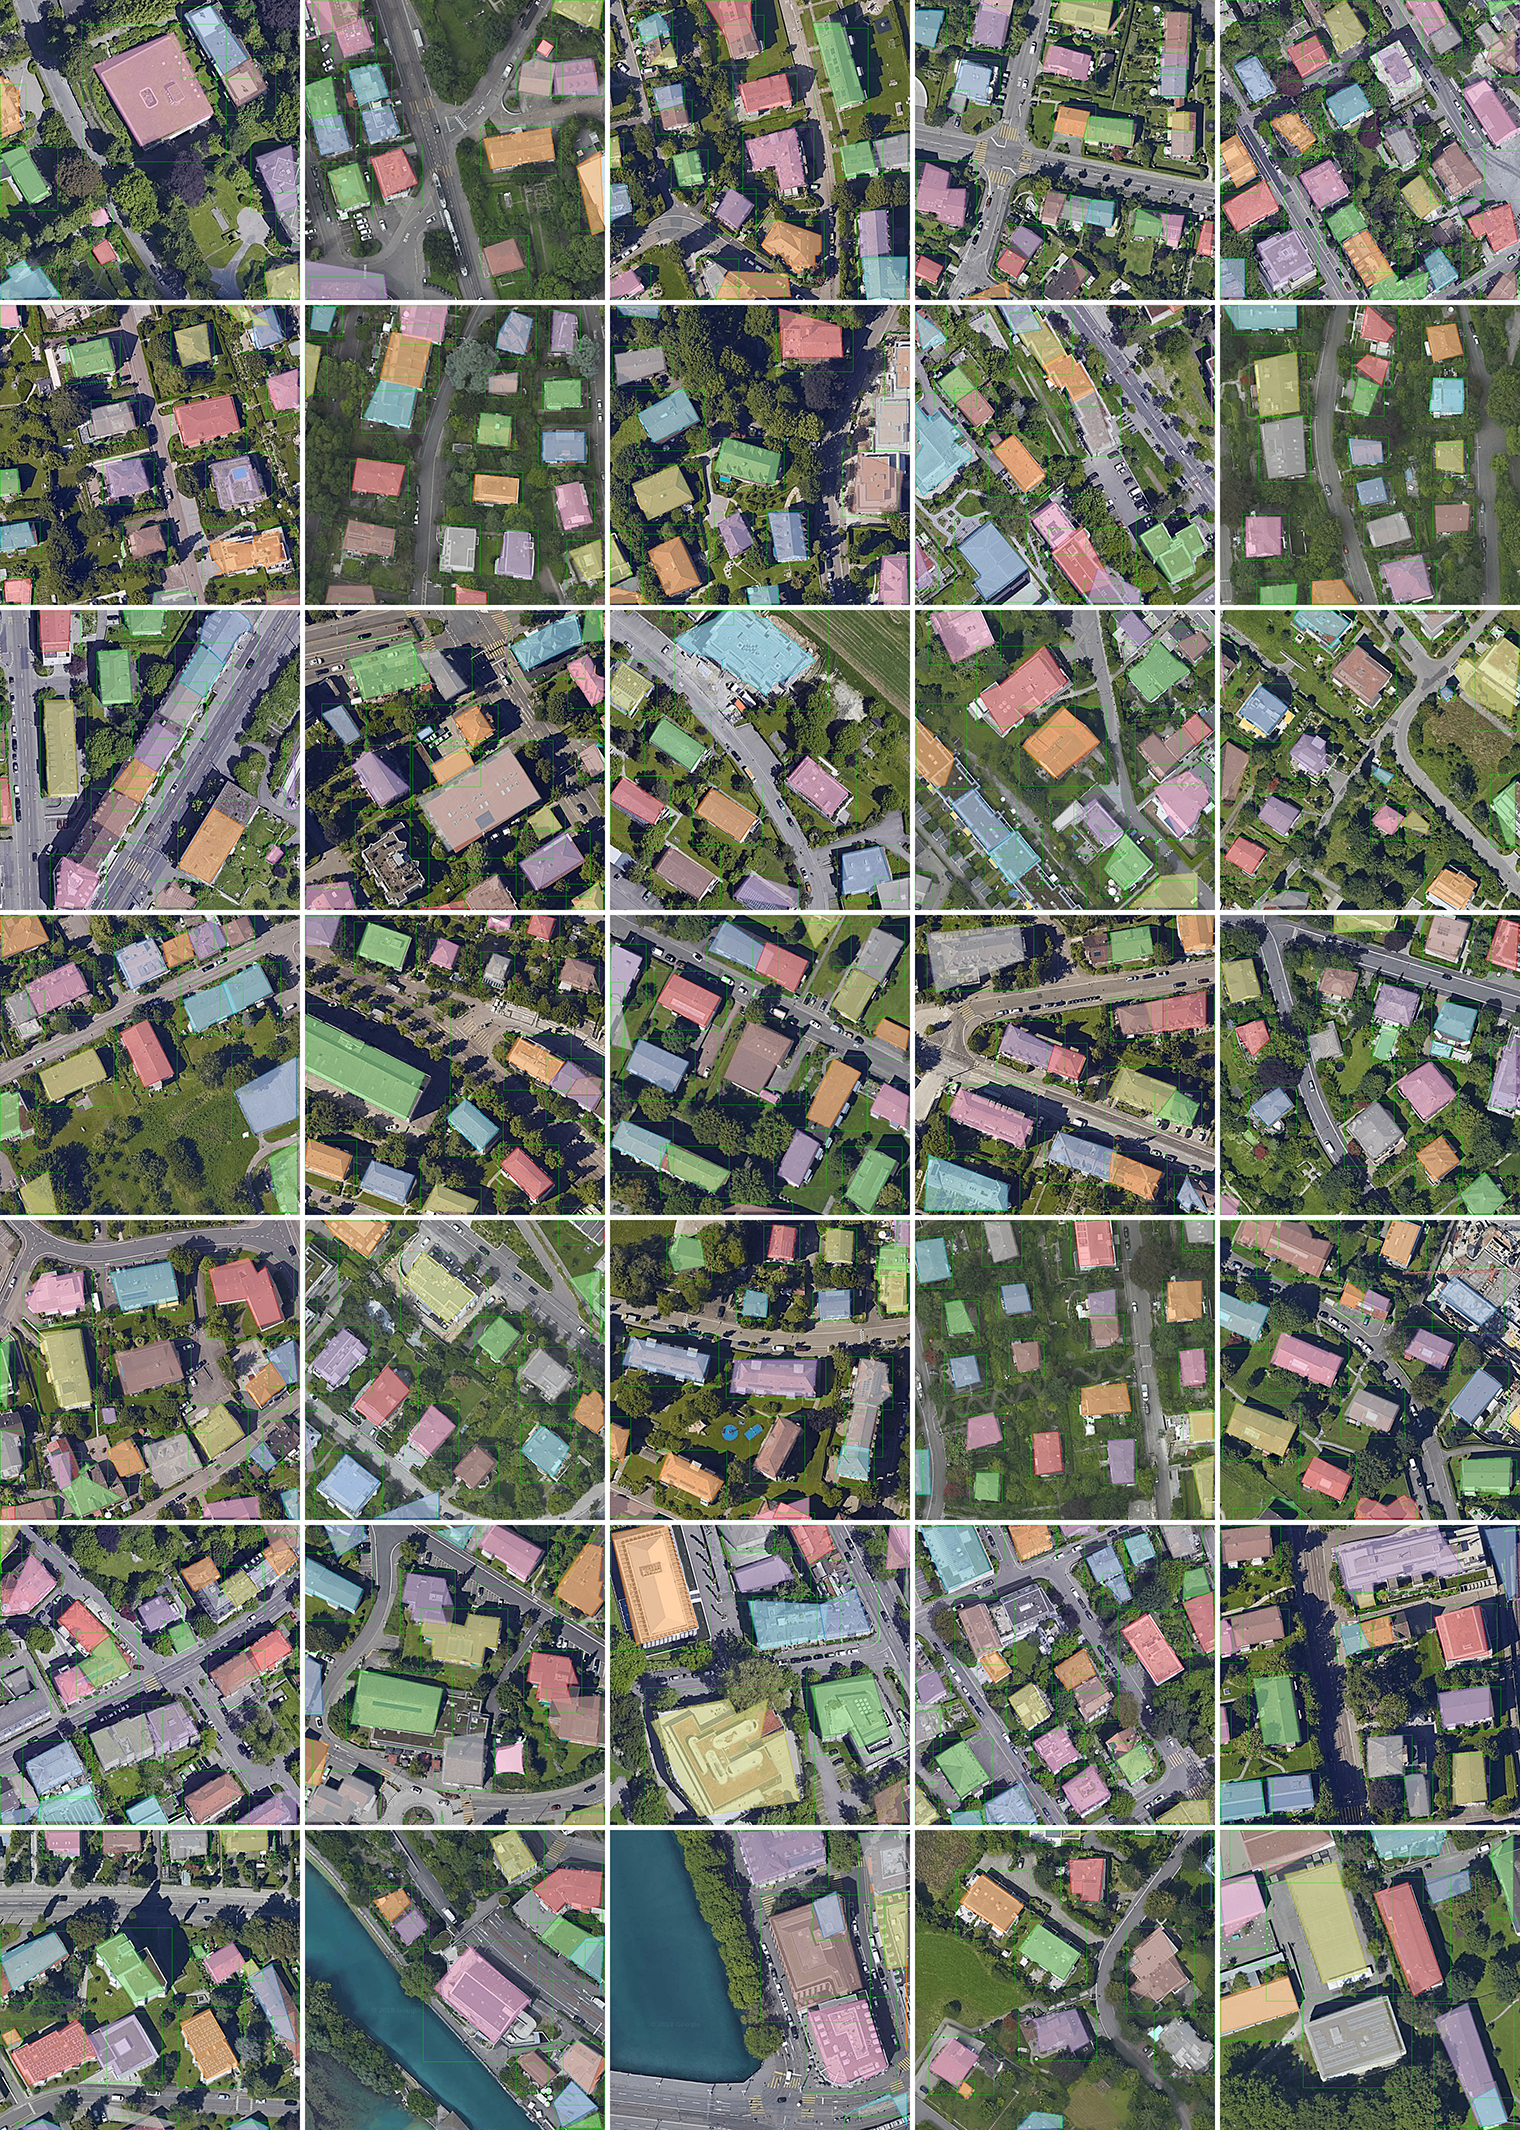
\includegraphics[width=\fig\textwidth]{6-00.png}
    \caption[More prediction results on the test set of Zurich]{More prediction results on the test set of Zurich. Note that multiple colors are used here to differentiate building instances.}
	\label{fig:finalzhmore}
\end{figure}

\section{Chicago}\label{app:predch}
Figure \ref{fig:finalchmore} gives more examples of prediction results in the test set of Chicago. Please zoom in for more details.
\begin{figure}[!h]
	\centering
	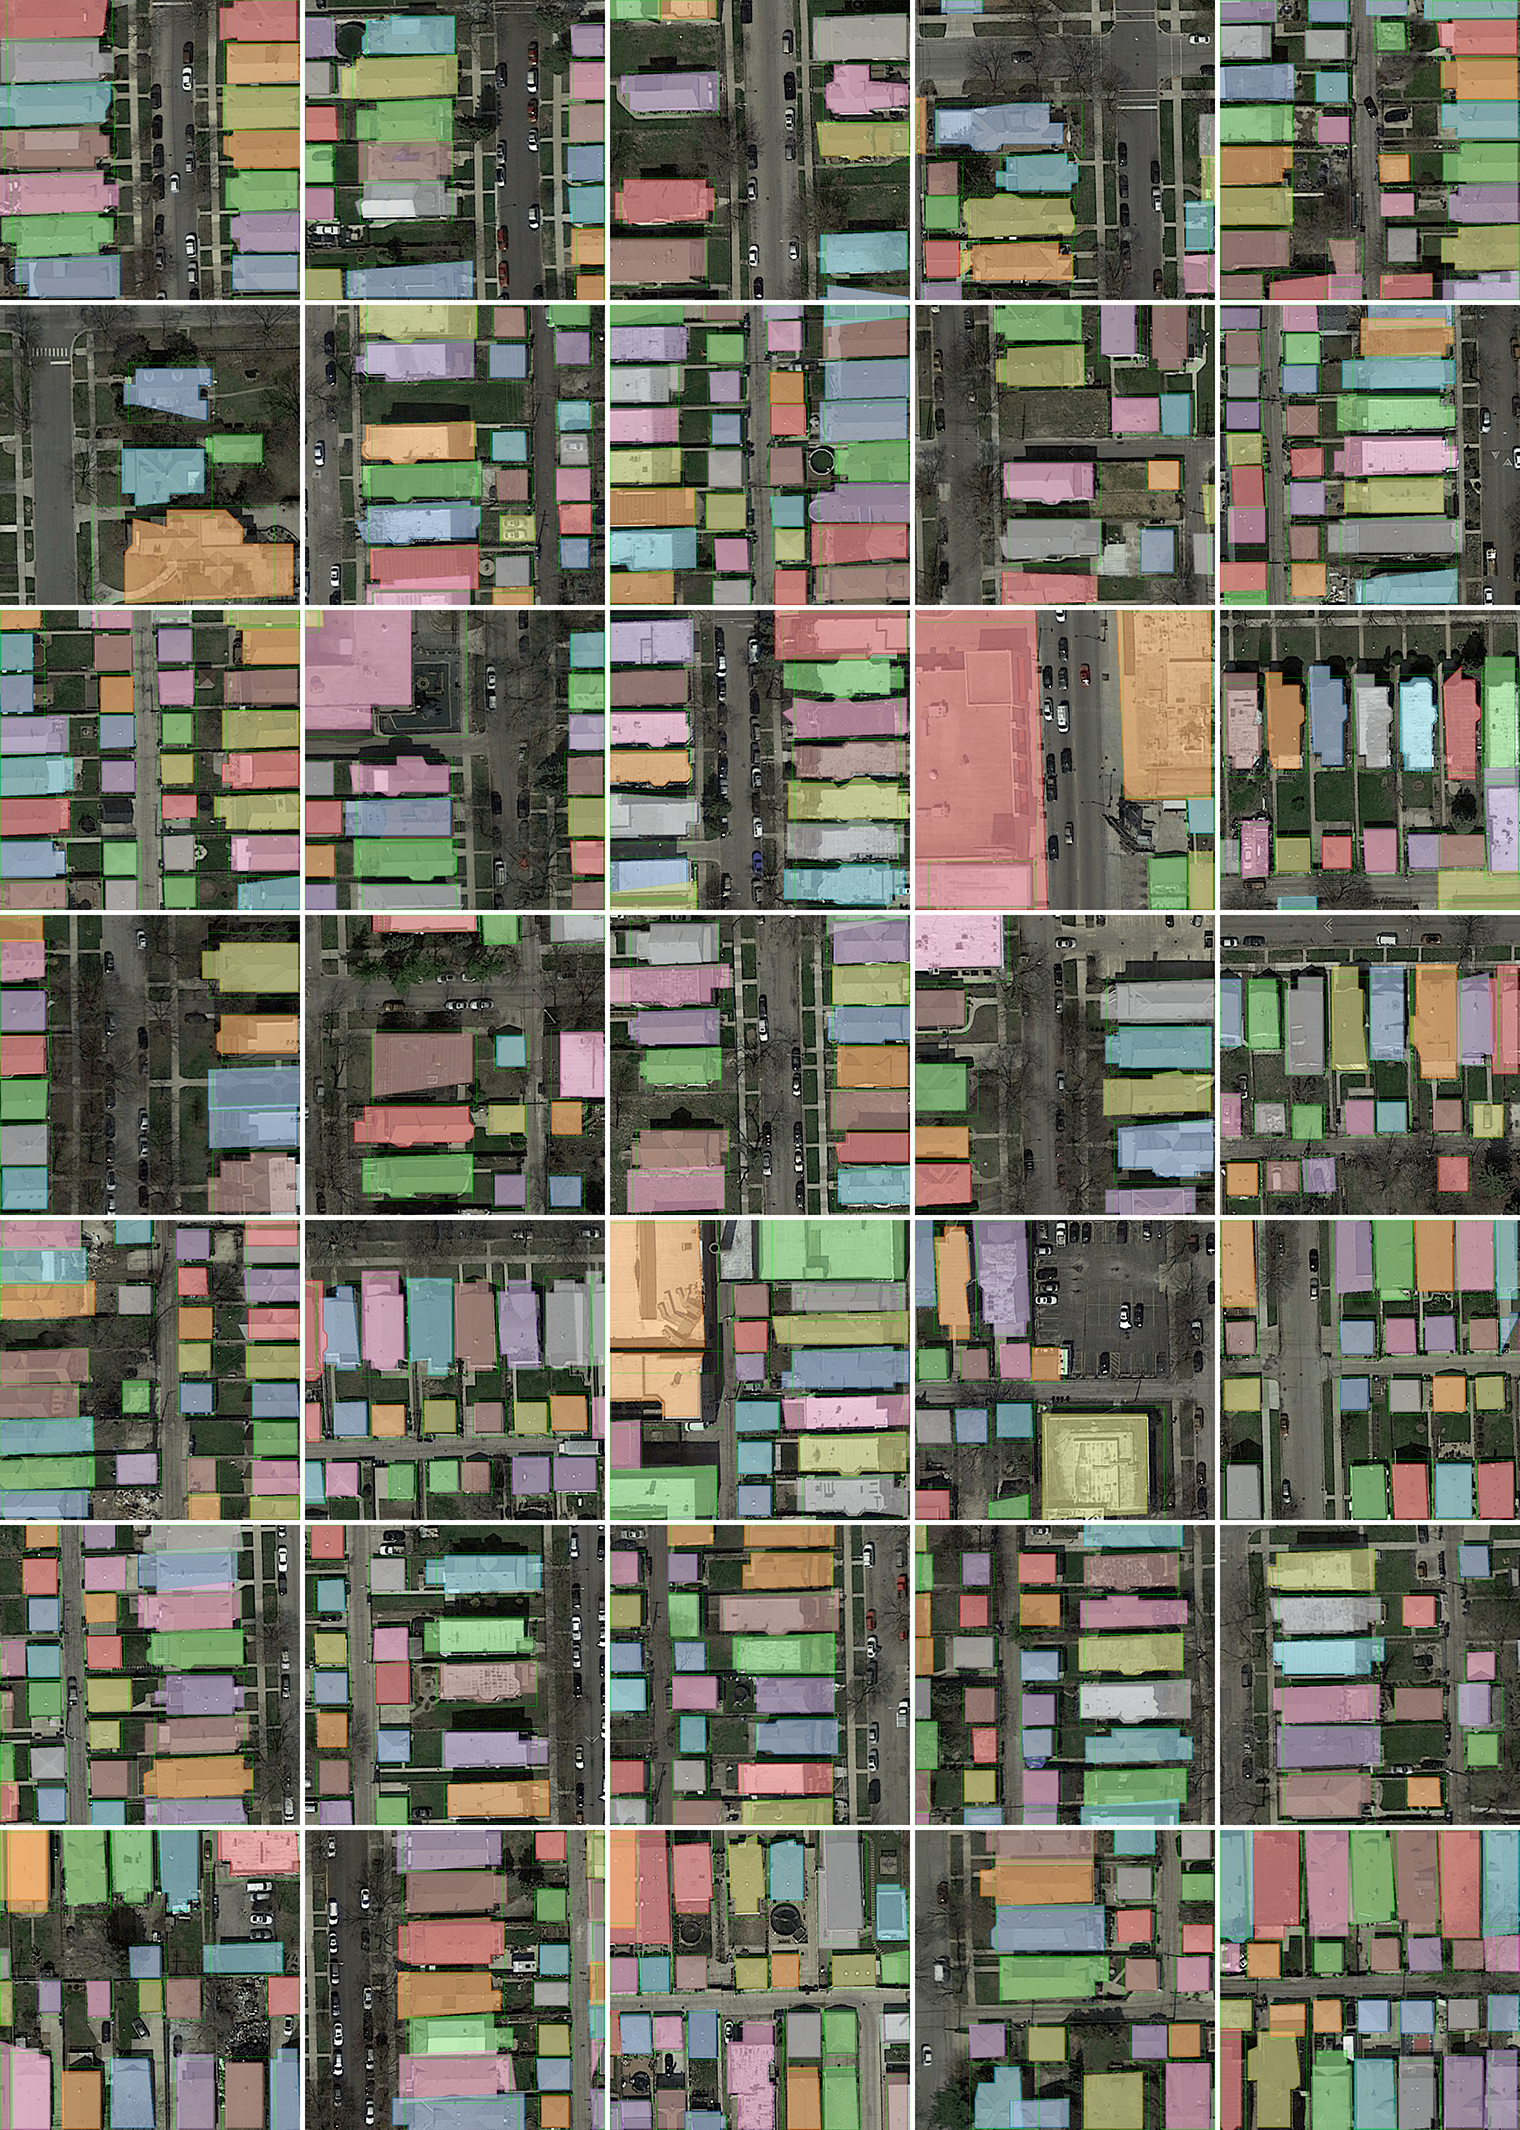
\includegraphics[width=\fig\textwidth]{6-01.png}
    \caption[More prediction results on the test set of Chicago]{More prediction results on the test set of Chicago. Note that multiple colors are used here to differentiate building instances.}
	\label{fig:finalchmore}
\end{figure}